% ==============================================================================
% Dynamic Narrative Personalization in Games Using AI
% Research Paper — IEEE Conference Format
% ==============================================================================
\documentclass[conference]{IEEEtran}
\IEEEoverridecommandlockouts
% The preceding line is only needed to identify funding in the first footnote.
% If that is unneeded, please comment it out.
\usepackage{cite}
\usepackage{amsmath,amssymb,amsfonts}
\usepackage{algorithmic}
\usepackage{graphicx}
\usepackage{textcomp}
\usepackage{xcolor}
\usepackage{booktabs}
\usepackage{tikz}
\usepackage{pgfplots}
\pgfplotsset{compat=1.18}
\usetikzlibrary{positioning, arrows.meta, fit, backgrounds}
\usepackage{subcaption}
\usepackage{hyperref}
\usepackage{balance}
\def\BibTeX{{\rm B\kern-.05em{\sc i\kern-.025em b}\kern-.08em
    T\kern-.1667em\lower.7ex\hbox{E}\kern-.125emX}}

\hypersetup{
    colorlinks=true,
    linkcolor=black,
    citecolor=blue!60!black,
    urlcolor=blue!60!black
}

% ── Title ──
\title{Dynamic Narrative Personalization in Games: A Closed-Loop System Using Player Modelling and RL-Guided LLM Generation}

\author{
    \IEEEauthorblockN{1\textsuperscript{st} Rivindu Bopage}
    \IEEEauthorblockA{
        \textit{School of Computing} \\
        \textit{Robert Gordon University} \\
        Aberdeen, United Kingdom \\
        r.bopage@rgu.ac.uk
    }
}

\begin{document}

\maketitle

% ==============================================================================
% ABSTRACT
% ==============================================================================
\begin{abstract}
Current game narrative systems deliver the same story to every player regardless of how they play. We present a closed-loop Unity plugin that personalises RPG narrative in real time by integrating five modules: (1)~telemetry-derived Hexad-analogous player profiling from 23 behavioural signals, (2)~a rule-based Flow state classifier, (3)~a PPO reinforcement learning agent that selects among eight narrative tone actions, (4)~a RAG-grounded local LLM (Phi-3.5 Mini) for lore-consistent text generation, and (5)~importance-weighted episodic session memory. A between-subjects user study ($N = 49$; 25 Experimental, 24 Control) using the Game Experience Questionnaire, a custom Narrative Personalization Scale (NPS-3), and semi-structured interviews found that the adaptive system produced significantly higher perceived personalization ($d = 0.84$, $p = .005$), a medium effect on Flow ($d = 0.65$, $p = .027$), and no significant effect on immersion ($d = 0.38$). Behavioural telemetry corroborated the self-report findings: Experimental participants read 72\% of narrative dialogue versus 58\% in the Control condition ($d = 0.87$). Reflexive Thematic Analysis of 20 interviews identified four themes, including ambient narrative responsiveness and occasional tone--state dissonance as a failure mode. The system demonstrates the feasibility of integrating continuous player modelling, RL-based narrative adaptation, and constrained LLM generation within a single real-time game pipeline.
\end{abstract}

\begin{IEEEkeywords}
narrative personalization, player modelling, reinforcement learning, large language models, retrieval-augmented generation, flow theory, dynamic difficulty adjustment, game AI
\end{IEEEkeywords}

% ==============================================================================
% I. INTRODUCTION
% ==============================================================================
\section{Introduction}

Games are the only narrative medium in which the audience both directs the protagonist and shapes how the story unfolds. Yet most commercially released games present nearly the same narrative sequence to every player. The village elder delivers the same warning whether the player is a careful explorer or a reckless disruptor who skips dialogue and rushes into combat.

This uniformity stems not from lack of interest but from the cost of creating alternatives. Each authored branch demands additional writing, voice work, and implementation, growing at a combinatorial rate. Even narratively ambitious titles like \textit{Disco Elysium} hit a practical upper limit on authored branching long before achieving genuinely player-adaptive personalization.

The convergence of large language models (LLMs) capable of coherent long-form text~\cite{brown2020language}, real-time player behaviour modelling, and reinforcement learning (RL) policy optimisation points to a new opportunity: narrative generated on the fly in response to an individual player's observed preferences and engagement profile. Prior work has addressed components of this problem in isolation. PANGeA~\cite{todd2024pangea} demonstrated LLM-grounded narrative generation but without a player model or adaptive policy. LIGS~\cite{ligs2025chi} addressed narrative coherence across sessions but not personalization. DDA systems~\cite{hunicke2004ai, climent2024framework} adapt mechanical parameters (enemy health, spawn rates) but not story content. No prior system has integrated continuous player profiling, Flow-based RL reward shaping, RAG-grounded LLM generation, and episodic session memory into a single closed-loop pipeline.

This paper presents such a system: a Unity plugin that continuously profiles the player using telemetry-derived Hexad-analogous scores~\cite{tondello2016hexad} and a Flow state classifier based on Csikszentmihalyi's~\cite{csikszentmihalyi1990flow} challenge--skill balance framework. A PPO agent~\cite{schulman2017proximal} selects among eight narrative actions; a RAG pipeline constrains the LLM to a structured lore corpus; and an episodic memory module maintains cross-event narrative coherence. We evaluate the system in a between-subjects study ($N = 49$) using validated psychometric instruments and behavioural telemetry.

\textbf{Contributions.} (1)~A method for deriving continuous Hexad-analogous behavioural motivation scores from in-session telemetry without a pre-play questionnaire. (2)~A RAG pipeline that selects lore context dynamically based on player state. (3)~Importance-weighted episodic session memory for cross-event narrative continuity. (4)~A feasibility demonstration of PPO for narrative action selection using a Flow-based MDP reward. (5)~A mixed-methods evaluation showing significant personalization effects and corroborating behavioural evidence.

% ==============================================================================
% II. RELATED WORK
% ==============================================================================
\section{Related Work}

\subsection{Narrative Personalization}

Drama management systems~\cite{mateas2003facade} showed that AI could reshape narrative arcs around player behaviour, but required every intervention to be hand-authored. Procedural narrative generation (Tracery~\cite{compton2015tracery}, Expressionist~\cite{kreminski2019evaluating}) produced varied text but had no mechanism for sensing the player's psychological state. Short~\cite{short2019procedural} crystallised the critique: procedural generation without a player intent model produces content that is varied but meaningless. Commercial branching systems (\textit{Mass Effect}, \textit{Disco Elysium}) respond only to explicit choices, not to implicit behavioural signals.

\subsection{Player Modelling}

Bartle's~\cite{bartle1996hearts} four-type taxonomy was foundational but categorical and static. Yee~\cite{yee2006motivations} showed that motivation is continuous and multi-dimensional. Tondello et al.~\cite{tondello2016hexad} addressed this with the Hexad scale, grounded in Self-Determination Theory~\cite{ryan2000self}, providing six continuous dimensions. However, the Hexad scale is a 24-item \textit{pre-play} questionnaire---a static snapshot that cannot update during a session. Our system infers Hexad-analogous scores directly from behavioural telemetry, updating continuously within the session.

\subsection{Flow Theory and DDA}

Csikszentmihalyi's~\cite{csikszentmihalyi1990flow} theory posits that optimal experience arises at the intersection of high challenge and high skill. Chen~\cite{chen2007flow} connected this to game design, arguing that many DDA mechanisms are implicit Flow-optimization systems. Hunicke and Chapman~\cite{hunicke2004ai} demonstrated adaptive difficulty's impact on retention. Climent et al.~\cite{climent2024framework} formalised RL-based DDA for single-player action games using PPO. However, DDA adapts \textit{mechanical} parameters exclusively; it does not adapt what the \textit{story does}.

\subsection{LLMs and RAG for Game Narrative}

PANGeA~\cite{todd2024pangea} generates coherent in-world narrative via LLM with prompt-grounded context, but its generation is procedural (driven by game state) rather than personalised (driven by player psychology). Ashby et al.~\cite{ashby2023personalized} used knowledge graphs for quest generation without real-time player modelling. V\"artinen et al.~\cite{vartinen2024generating} showed GPT-class models can generate complete RPG quest structures rated comparably to hand-authored content. RAG~\cite{lewis2020retrieval} keeps generation lore-consistent by injecting retrieved passages into the prompt at generation time.

\subsection{Gap Summary}

Table~\ref{tab:related_work} maps nine prior systems against six dimensions. No prior work covers more than three; the present system addresses all six.

\begin{table}[htbp]
\centering
\caption{Related work coverage across six system dimensions.}
\label{tab:related_work}
\scriptsize
\begin{tabular}{@{}lccccccc@{}}
\toprule
\textbf{System} & \textbf{Ref.} & \rotatebox{70}{\textbf{Player Model}} & \rotatebox{70}{\textbf{Flow Reward}} & \rotatebox{70}{\textbf{LLM Gen.}} & \rotatebox{70}{\textbf{RAG}} & \rotatebox{70}{\textbf{Ep. Memory}} & \rotatebox{70}{\textbf{Closed Loop}} \\
\midrule
PANGeA & \cite{todd2024pangea} & -- & -- & \checkmark & $\sim$ & -- & -- \\
LIGS & \cite{ligs2025chi} & -- & -- & \checkmark & -- & $\sim$ & -- \\
KG-Quest & \cite{ashby2023personalized} & -- & -- & \checkmark & KG & -- & -- \\
DDA & \cite{hunicke2004ai} & Beh. & Imp. & -- & -- & -- & -- \\
RL-DDA & \cite{climent2024framework} & Beh. & Imp. & -- & -- & -- & -- \\
player2vec & \cite{devlin2024player2vec} & Deep & -- & -- & -- & -- & -- \\
EM-LLM & \cite{fountas2024episodic} & -- & -- & \checkmark & -- & \checkmark & -- \\
\textbf{Ours} & & \textbf{Hex+} & \textbf{Exp.} & \checkmark & \checkmark & \checkmark & \checkmark \\
\bottomrule
\end{tabular}
\end{table}

% ==============================================================================
% III. SYSTEM ARCHITECTURE
% ==============================================================================
\section{System Architecture}

The system comprises five modules in a closed-loop pipeline (Fig.~\ref{fig:architecture}): telemetry collection (Unity), player modelling, PPO-based adaptation, RAG-grounded narrative generation, and content injection (Unity). The pipeline cycles every five seconds.

\begin{figure}[htbp]
\centering
\resizebox{\columnwidth}{!}{%
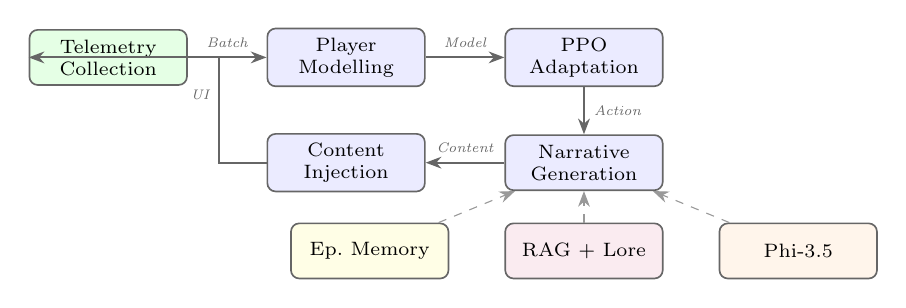
\begin{tikzpicture}[
    node distance=0.6cm and 1.0cm,
    >={Stealth[length=2mm]},
    mod/.style={rectangle, rounded corners=3pt, draw=black!60, line width=0.6pt, fill=#1, minimum width=2.0cm, minimum height=0.7cm, align=center, font=\scriptsize},
    mod/.default={blue!8},
    arr/.style={->, line width=0.7pt, black!60},
    lbl/.style={font=\tiny\itshape, text=black!60}
]
\node[mod=green!10] (tel) {Telemetry\\Collection};
\node[mod, right=of tel] (pm) {Player\\Modelling};
\node[mod, right=of pm] (ppo) {PPO\\Adaptation};
\node[mod, below=of ppo] (nar) {Narrative\\Generation};
\node[mod, left=of nar] (inj) {Content\\Injection};

\draw[arr] (tel) -- node[lbl, above] {Batch} (pm);
\draw[arr] (pm) -- node[lbl, above] {Model} (ppo);
\draw[arr] (ppo) -- node[lbl, right] {Action} (nar);
\draw[arr] (nar) -- node[lbl, above] {Content} (inj);
\draw[arr] (inj.west) -- +(-0.6,0) |- node[lbl, above left, pos=0.25] {UI} (tel.west);

\node[mod=purple!8, below=0.4cm of nar] (rag) {\scriptsize RAG + Lore};
\node[mod=orange!8, right=0.7cm of rag] (llm) {\scriptsize Phi-3.5};
\node[mod=yellow!10, left=0.7cm of rag] (mem) {\scriptsize Ep.\ Memory};

\draw[->, dashed, black!40] (rag) -- (nar);
\draw[->, dashed, black!40] (llm) -- (nar);
\draw[->, dashed, black!40] (mem) -- (nar);

\end{tikzpicture}%
}
\caption{Closed-loop system architecture. The pipeline cycles every five seconds from telemetry through adaptive narrative generation back to in-game delivery.}
\label{fig:architecture}
\end{figure}

\subsection{Telemetry Collection}

The Unity \texttt{PlayerDataLogger} captures 23 behavioural fields per five-second window (kills, deaths, damage, abilities, objectives, exploration, NPC interactions, dialogue engagement, lore items, idle time, and session metadata) and transmits a \texttt{TelemetryBatch} to the FastAPI backend via HTTP POST.

\subsection{Player Modelling}

The \textbf{Feature Extractor} computes 11 normalised scalar features from raw telemetry, including \texttt{kd\_ratio}, \texttt{objective\_rate}, \texttt{explore\_rate}, \texttt{dialogue\_engage}, \texttt{ability\_accuracy}, and a composite \texttt{challenge\_skill\_ratio} that operationalises Csikszentmihalyi's balance axis.

The \textbf{Hexad Profiler} derives six continuous scores $\in [0,1]$ from the cumulative session telemetry, each corresponding to a Hexad dimension (Achiever, Explorer, Socializer, Free Spirit, Disruptor, Philanthropist). These scores are behavioural motivation proxies inferred from telemetry patterns theoretically associated with each dimension, not validated Hexad questionnaire equivalents.

The \textbf{Flow Classifier} assigns one of four states via a rule-based decision tree:
\begin{itemize}
    \item \textbf{APATHY}: idle $> 0.4$ AND dialogue\_engage $< 0.3$ AND ratio $< 0.75$
    \item \textbf{BOREDOM}: ratio $< 0.75$
    \item \textbf{ANXIETY}: ratio $> 1.30$
    \item \textbf{FLOW}: ratio $\in [0.75, 1.30]$
\end{itemize}
The thresholds define a zone around challenge--skill balance ($= 1.0$), with asymmetry ($-0.25$ below, $+0.30$ above) reflecting that players tolerate slight over-challenge better than under-challenge~\cite{yannakakis2009realtime}. These are design parameters, not empirically calibrated values.

\subsection{PPO-Based Narrative Adaptation}

The adaptation problem is formalised as an MDP $(S, A, T, R, \gamma)$:

\textbf{State space $S$:} A 7-dimensional continuous vector: encoded Flow state, normalised challenge--skill ratio, four Hexad dimensions (Explorer, Socializer, Achiever, Disruptor), and normalised session progress. Free Spirit and Philanthropist are excluded as a deliberate dimensionality reduction; their signals are captured by other state components.

\textbf{Action space $A$:} Discrete(8) corresponding to eight narrative actions: \textsc{Lower\_Stakes}, \textsc{Raise\_Stakes}, \textsc{Add\_Mystery}, \textsc{Add\_Humor}, \textsc{Provide\_Guidance}, \textsc{Increase\_Urgency}, \textsc{Lore\_Reward}, and \textsc{No\_Change}.

\textbf{Reward function $R$:} The reward directly operationalises Flow theory with graduated penalties: FLOW $= +1.0$, BOREDOM $= -0.3$, ANXIETY $= -0.5$, APATHY $= -0.8$. Shaping rewards include a Flow streak bonus ($+0.20$ after two consecutive FLOW steps), a transition bonus ($+0.30$ for recovering from ANXIETY/BOREDOM to FLOW), a repetition penalty ($-0.15$ when all three recent actions are identical), and a step penalty ($-0.05$). These values are hand-tuned hyperparameters; the graduated ordering follows the theoretical rationale that deeper disengagement is harder to recover from~\cite{csikszentmihalyi1990flow, chen2007flow}. The shaping rewards follow the principle of potential-based reward shaping~\cite{ng1999policy}.

The agent uses Stable-Baselines3~\cite{raffin2021stable} PPO with MlpPolicy (two hidden layers of 64 units), trained for 200,000 timesteps in a simulated Gymnasium environment. For the first 120 seconds of a session, a deterministic cold-start heuristic maps Flow states to actions (ANXIETY $\to$ \textsc{Provide\_Guidance}, BOREDOM $\to$ \textsc{Increase\_Urgency}, APATHY $\to$ \textsc{Add\_Mystery}, FLOW $\to$ \textsc{No\_Change}).

\subsection{RAG-Grounded Narrative Generation}

The \texttt{LoreRetriever} uses sentence-transformers all-MiniLM-L6-v2~\cite{wang2020minilm} to embed a lore corpus (world, character, and quest documents) into a 384-dimensional space. At generation time, the top $k=3$ passages by cosine similarity are retrieved and injected into the prompt alongside the selected narrative action, the player model summary, and the episodic memory context.

\subsection{Episodic Session Memory}

Inspired by EM-LLM~\cite{fountas2024episodic}, a lightweight memory module maintains up to ten narrative events tagged with importance scores $\in [0,1]$. When capacity is exceeded, the least important event is evicted. At generation time, the top five events by importance are included in the prompt, enabling cross-event references and character continuity.

% ==============================================================================
% IV. EVALUATION
% ==============================================================================
\section{Evaluation}

\subsection{Study Design}

A between-subjects design with random assignment ($N = 50$; 1 excluded due to server crash, yielding $N = 49$: 25 Experimental, 24 Control). The Experimental condition deployed the full adaptive system; the Control condition replaced adaptive narrative with a \texttt{StaticNarrativeContent} asset delivering pre-authored fragments. All other aspects (game environment, objectives, UI, session duration of 30 minutes) were identical across conditions. The testbed was a 3D RPG built on the AnyRPG Core framework in Unity 2021.3 LTS.

\subsection{Instruments}

\textbf{GEQ Core Module}~\cite{ijsselsteijn2013geq}: 33-item, 0--4 scale. Primary DV: Flow subscale (5 items, $\alpha = .79$). Secondary DV: Immersion subscale (6 items, $\alpha = .82$).

\textbf{NPS-3}: Custom 3-item Narrative Personalization Scale (1--7 Likert, $\alpha = .76$). As a custom instrument without independent validation, the NPS-3 result is best interpreted as evidence of perceived narrative responsiveness rather than a validated personalization measure.

\textbf{miniPXI}~\cite{vornhagen2022minipxi}: 11-item, 1--7 scale. Total score as a general player experience index.

\textbf{Semi-structured interviews}: 20 participants (10 per condition), analysed via Reflexive Thematic Analysis~\cite{braun2022thematic}.

\subsection{Statistical Approach}

Welch's $t$-tests with Bonferroni correction across three hypotheses ($\alpha_{\text{adj}} = .0167$). Effect sizes reported as Cohen's $d$. A priori power analysis (G*Power~\cite{faul2007gpower}) targeting $d = 0.5$, $\alpha = .05$, power $= 0.80$ indicated $n = 25$ per group.

% ==============================================================================
% V. RESULTS
% ==============================================================================
\section{Results}

\subsection{Participants}

The final sample ($N = 49$) was predominantly male (65\%), mean age 22.2 ($SD = 2.2$), mean gaming hours 13.1/week ($SD = 6.7$). No significant baseline differences between conditions on age ($p = .42$) or gaming hours ($p = .71$).

\subsection{Hypothesis Tests}

Table~\ref{tab:results} summarises the primary results.

\begin{table}[htbp]
\centering
\caption{Primary hypothesis test results.}
\label{tab:results}
\scriptsize
\begin{tabular}{@{}llllll@{}}
\toprule
\textbf{Measure} & \textbf{Exp.\ $M$ ($SD$)} & \textbf{Ctrl.\ $M$ ($SD$)} & $t$ & $p$ & $d$ \\
\midrule
GEQ Flow & 2.78 (0.62) & 2.36 (0.68) & 2.28 & .027 & 0.65 \\
GEQ Imm. & 2.64 (0.71) & 2.38 (0.66) & 1.34 & .187 & 0.38 \\
NPS-3 & 4.92 (1.18) & 3.88 (1.31) & 2.94 & .005$^{**}$ & 0.84 \\
\bottomrule
\multicolumn{6}{l}{\scriptsize $^{**}$ Survives Bonferroni correction ($\alpha_{\text{adj}} = .0167$).}
\end{tabular}
\end{table}

\textbf{H1 (Flow):} Partially supported. The Experimental group reported higher GEQ Flow ($d = 0.65$, medium), but the result narrowly missed the Bonferroni threshold ($p = .027 > .0167$).

\textbf{H2 (Immersion):} Not supported ($d = 0.38$, $p = .187$).

\textbf{H3 (Personalization):} Strongly supported. NPS-3 scores were significantly higher in the Experimental condition ($d = 0.84$, large), surviving Bonferroni correction ($p = .005$).

\subsection{Behavioural Metrics}

Experimental participants read a significantly higher proportion of narrative dialogue ($M = 0.72$ vs.\ $0.58$, $d = 0.87$, $p = .004$) and initiated more voluntary NPC interactions ($M = 8.4$ vs.\ $6.2$, $d = 0.75$, $p = .012$). These behavioural indicators are immune to demand characteristics and provide demand-characteristic-free corroboration of the self-report findings.

\subsection{Qualitative Themes}

Reflexive Thematic Analysis~\cite{braun2022thematic} of 20 interviews yielded four themes:

\textbf{Theme 1: ``The story pays attention.''} Eight of 10 Experimental interviewees described an ambient sense that the narrative responded to their behaviour, using metaphors of being ``noticed'' by the game.

\textbf{Theme 2: ``Tone matching.''} Six Experimental participants described specific moments where narrative tone aligned with gameplay intensity.

\textbf{Theme 3: ``Generic narrative as wallpaper.''} Seven of 10 Control interviewees described gradual disengagement from narrative content, consistent with the lower dialogue read ratio.

\textbf{Theme 4: ``Occasional dissonance.''} Four Experimental participants noted moments of tone mismatch, typically receiving ``mystery'' content during intense combat. This identifies a concrete failure mode: the 5-second telemetry cycle causes the PPO agent's action selection to lag behind rapid state transitions.

% ==============================================================================
% VI. DISCUSSION
% ==============================================================================
\section{Discussion}

The pattern of results---strong personalization ($d = 0.84$), moderate Flow ($d = 0.65$), weak immersion ($d = 0.38$)---is internally coherent. The system directly manipulates narrative content in response to player state (captured by NPS-3), producing a downstream effect on Flow (the PPO optimisation target), but not reaching the broader construct of immersion, which depends on production values outside the system's control.

The behavioural metrics substantially strengthen the quantitative interpretation. Participants did not know their dialogue reading behaviour was being measured, so the difference ($d = 0.87$) cannot be attributed to response bias. The adaptive narrative changed what participants \textit{did} during play, not merely what they \textit{said} about it afterward.

The qualitative themes provide mechanistic insight: Theme~2 (tone matching) reflects effective PPO action selection, while Theme~4 (dissonance) identifies the 5-second telemetry cycle as a design limitation rather than a policy failure. No participants in either condition described the narrative as obviously AI-generated, consistent with LIGS's finding~\cite{ligs2025chi} that constrained LLM output can be subjectively indistinguishable from human-authored content.

\subsection{Limitations}

The PPO agent was trained on a simulated MDP with hand-specified transitions; the learned policy reflects simulator assumptions, not empirical player dynamics. The contribution is therefore a feasibility demonstration, not a claim of policy optimality. The Hexad profiling is rule-based and unvalidated against questionnaire ground truth. The NPS-3 is a custom instrument without independent validation ($\alpha = .76$). The LLM (Phi-3.5 Mini, 3.8B) constrains narrative quality. The single 30-minute session captures no cumulative effects, and the testbed game is a simplified prototype, not a commercial title. With $n = 25$ per condition, the study detects medium-to-large effects but would miss small ones.

% ==============================================================================
% VII. CONCLUSION AND FUTURE WORK
% ==============================================================================
\section{Conclusion}

This paper presented a closed-loop system that personalises RPG narrative in real time using telemetry-derived player profiling, PPO-based narrative action selection, RAG-grounded LLM generation, and episodic session memory. A between-subjects evaluation ($N = 49$) found strong evidence for perceived personalization ($d = 0.84$), partial evidence for enhanced Flow ($d = 0.65$), and corroborating behavioural evidence ($d = 0.87$ for dialogue engagement). The system demonstrates that continuous player modelling, RL-based narrative adaptation, and constrained LLM generation can be integrated into a single real-time game pipeline.

Future work should pursue empirical validation of telemetry-derived Hexad profiles against questionnaire ground truth, online RL adaptation with real player interaction data, evaluation with larger LLMs and in commercial game contexts, and longitudinal studies spanning multiple sessions.

% ==============================================================================
% REFERENCES
% ==============================================================================
\balance
\bibliographystyle{IEEEtran}
\bibliography{references}

\end{document}